\documentclass{standalone}

    \usepackage{tikz}
    \usetikzlibrary{arrows, automata, positioning, fit}
    \tikzset{
      reflexive above/.style={->,loop,looseness=7,in=60,out=120, above},
      reflexive below/.style={->,loop,looseness=7,in=300,out=240, below},
      reflexive left/.style={->,loop,looseness=7,in=150,out=210, left},
      reflexive right/.style={->,loop,looseness=7,in=30,out=330, right},
    }
    
\begin{document}
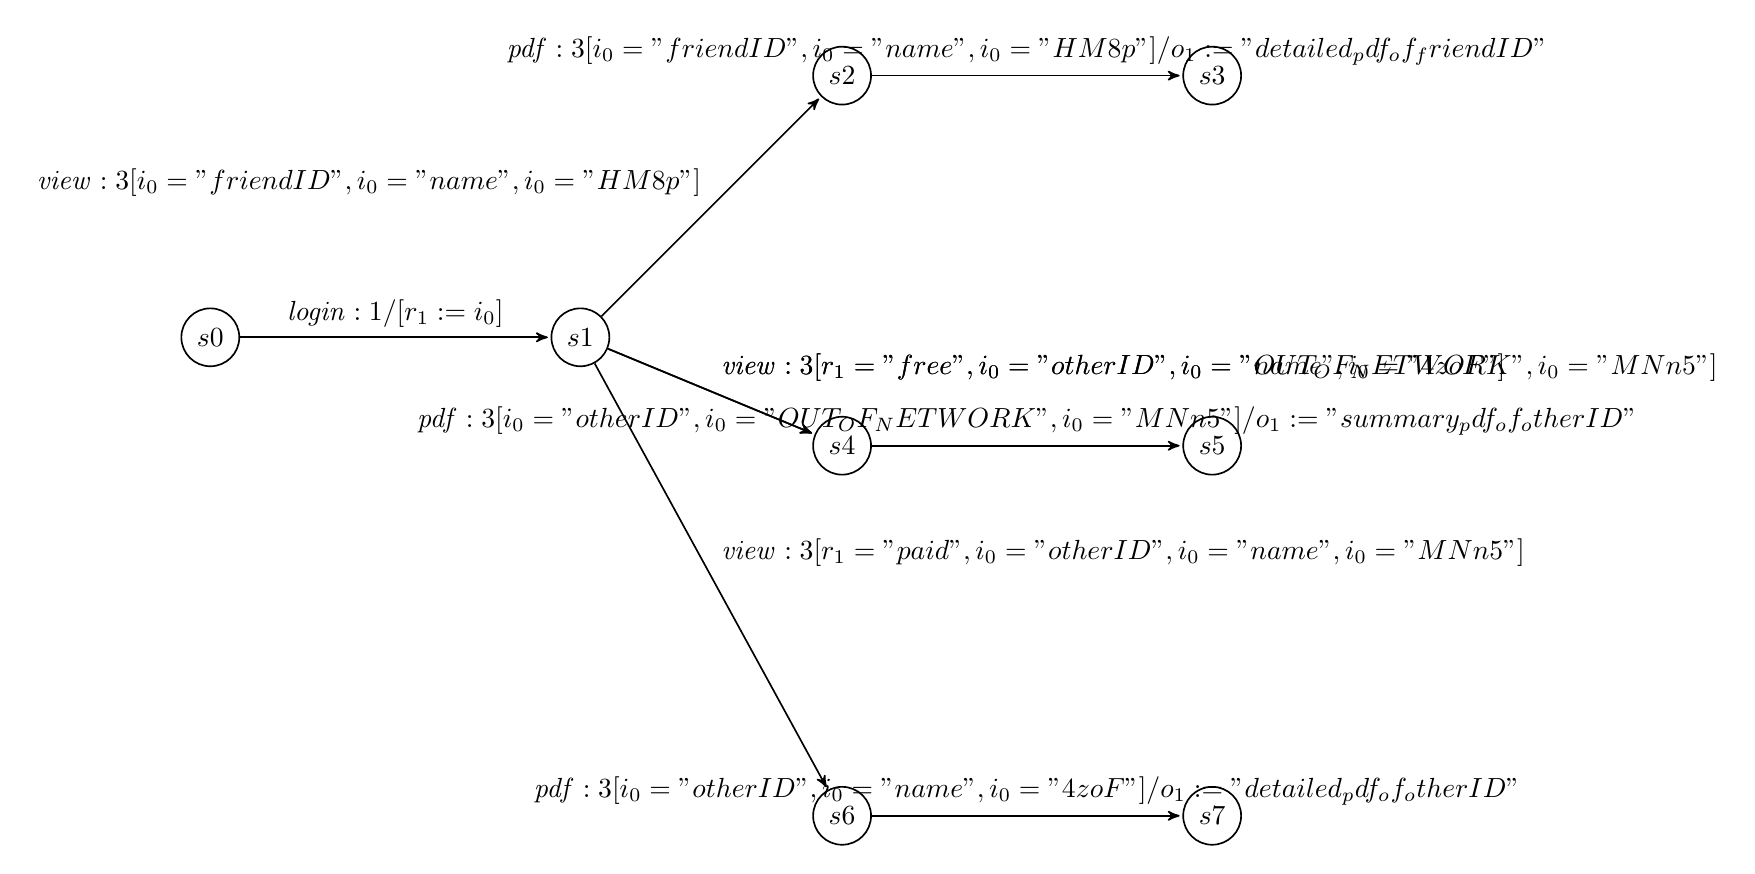
\begin{tikzpicture}[->,>=stealth',shorten >=1pt,auto,node distance=4.7cm,semithick, initial text={}, state/.style={circle, draw, minimum size=0.5cm}]
  \node[state] (s0) [] {$s0$};
  \node[state] (s1) [right of = s0] {$s1$};
  \node[state] (s2) [above right of = s1] {$s2$};
  \node[state] (s3) [right of = s2] {$s3$};
  \node[state] (s4) [below of = s2] {$s4$};
  \node[state] (s5) [right of = s4] {$s5$};
  \node[state] (s6) [below of = s4] {$s6$};
  \node[state] (s7) [right of = s6] {$s7$};

  \draw (s0) edge node{$\mathit{login}:1/[r_1 := i_0]$} (s1);
  \draw (s1) edge node{$\mathit{view}:3[i_0 = "friendID", i_0 = "name", i_0 = "HM8p"]$} (s2);
  \draw (s1) edge node{$\mathit{view}:3[r_1 = "free", i_0 = "otherID", i_0 = "OUT_OF_NETWORK", i_0 = "MNn5"]$} (s4);
  \draw (s1) edge node{$\mathit{view}:3[r_1 = "free", i_0 = "otherID", i_0 = "name", i_0 = "4zoF"]$} (s4);
  \draw (s1) edge node{$\mathit{view}:3[r_1 = "paid", i_0 = "otherID", i_0 = "name", i_0 = "MNn5"]$} (s6);
  \draw (s2) edge node{$\mathit{pdf}:3[i_0 = "friendID", i_0 = "name", i_0 = "HM8p"]/o_1 := "detailed_pdf_of_friendID"$} (s3);
  \draw (s4) edge node{$\mathit{pdf}:3[i_0 = "otherID", i_0 = "OUT_OF_NETWORK", i_0 = "MNn5"]/o_1 := "summary_pdf_of_otherID"$} (s5);
  \draw (s6) edge node{$\mathit{pdf}:3[i_0 = "otherID", i_0 = "name", i_0 = "4zoF"]/o_1 := "detailed_pdf_of_otherID"$} (s7);
\end{tikzpicture}
\end{document}
